% Project:			Mediation and Gender Differences
% This file:		Main writeup
% Original date: 	December 7, 2016

%Style
\documentclass[12pt]{article}
\usepackage[top=1in, bottom=1in, left=1in, right=1in]{geometry}
\parindent 22pt
\usepackage{fancyhdr}

%Packages
\usepackage{adjustbox}
\usepackage{amsmath}
\usepackage{amsfonts}
\usepackage{amssymb}
\usepackage{bm}
\usepackage[table]{xcolor}
\usepackage{tabu}
\usepackage{color,soul}
\usepackage{makecell}
\usepackage{longtable}
\usepackage{multirow}
\usepackage[normalem]{ulem}
\usepackage{etoolbox}
\usepackage{graphicx}
\usepackage{tabularx}
\usepackage{ragged2e}
\usepackage{booktabs}
\usepackage{caption}
\usepackage{fixltx2e}
\usepackage[para, flushleft]{threeparttablex}
\usepackage[capposition=top,objectset=centering]{floatrow}
\usepackage{subcaption}
\usepackage{pdfpages}
\usepackage{pdflscape}
\usepackage{natbib}
\usepackage{bibunits}
\definecolor{maroon}{HTML}{990012}
\usepackage[colorlinks=true,linkcolor=maroon,citecolor=maroon,urlcolor=maroon,anchorcolor=maroon]{hyperref}
\usepackage{marvosym}
\usepackage{makeidx}
\usepackage{tikz}
\usetikzlibrary{shapes}
\usepackage{setspace}
\usepackage{enumerate}
\usepackage{rotating}
\usepackage{tocloft}
\usepackage{epstopdf}
\usepackage[titletoc]{appendix}
\usepackage{framed}
\usepackage{comment}
\usepackage{xr}
\usepackage{titlesec}
\usepackage{footnote}
\usepackage{longtable}
\newlength{\tablewidth}
\setlength{\tablewidth}{9.3in}
\setcounter{secnumdepth}{4}

\titleformat{\paragraph}
{\normalfont\normalsize\bfseries}{\theparagraph}{1em}{}
\titlespacing*{\paragraph}
{0pt}{3.25ex plus 1ex minus .2ex}{1.5ex plus .2ex}
\makeatletter
\pretocmd\start@align
{%
  \let\everycr\CT@everycr
  \CT@start
}{}{}
\apptocmd{\endalign}{\CT@end}{}{}
\makeatother
%Watermark
\usepackage[printwatermark]{xwatermark}
\usepackage{lipsum}
\definecolor{lightgray}{RGB}{220,220,220}
%\newwatermark[allpages,color=lightgray,angle=45,scale=3,xpos=0,ypos=0]{Preliminary Draft}

%Further subsection level
\usepackage{titlesec}
\setcounter{secnumdepth}{4}
\titleformat{\paragraph}
{\normalfont\normalsize\bfseries}{\theparagraph}{1em}{}
\titlespacing*{\paragraph}
{0pt}{3.25ex plus 1ex minus .2ex}{1.5ex plus .2ex}

\setcounter{secnumdepth}{5}
\titleformat{\subparagraph}
{\normalfont\normalsize\bfseries}{\thesubparagraph}{1em}{}
\titlespacing*{\subparagraph}
{0pt}{3.25ex plus 1ex minus .2ex}{1.5ex plus .2ex}

%Functions
\DeclareMathOperator{\cov}{Cov}
\DeclareMathOperator{\corr}{Corr}
\DeclareMathOperator{\var}{Var}
\DeclareMathOperator{\plim}{plim}
\DeclareMathOperator*{\argmin}{arg\,min}
\DeclareMathOperator*{\argmax}{arg\,max}

%Math Environments
\newtheorem{theorem}{Theorem}
\newtheorem{claim}{Claim}
\newtheorem{condition}{Condition}
\renewcommand\thecondition{C--\arabic{condition}}
\newtheorem{algorithm}{Algorithm}
\newtheorem{assumption}{Assumption}
\renewcommand\theassumption{A--\arabic{assumption}}
\newtheorem{remark}{Remark}
\renewcommand\theremark{R--\arabic{remark}}
\newtheorem{definition}[theorem]{Definition}
\newtheorem{hypothesis}[theorem]{Hypothesis}
\newtheorem{property}[theorem]{Property}
\newtheorem{example}[theorem]{Example}
\newtheorem{result}[theorem]{Result}
\newenvironment{proof}{\textbf{Proof:}}{$\bullet$}

%Commands
\newcommand\independent{\protect\mathpalette{\protect\independenT}{\perp}}
\def\independenT#1#2{\mathrel{\rlap{$#1#2$}\mkern2mu{#1#2}}}
\newcommand{\overbar}[1]{\mkern 1.5mu\overline{\mkern-1.5mu#1\mkern-1.5mu}\mkern 1.5mu}
\newcommand{\equald}{\ensuremath{\overset{d}{=}}}
\captionsetup[table]{skip=10pt}
%\makeindex

\setlength\parindent{20pt}
\setlength{\parskip}{0pt}

\newcolumntype{L}[1]{>{\raggedright\let\newline\\\arraybackslash\hspace{0pt}}m{#1}}
\newcolumntype{C}[1]{>{\centering\let\newline\\\arraybackslash\hspace{0pt}}m{#1}}
\newcolumntype{R}[1]{>{\raggedleft\let\newline\\\arraybackslash\hspace{0pt}}m{#1}}



%Logo
%\AddToShipoutPictureBG{%
%  \AtPageUpperLeft{\raisebox{-\height}{
\includegraphics[width=1.5cm]{uchicago.png}}}
%}

\newcolumntype{L}[1]{>{\raggedright\let\newline\\\arraybackslash\hspace{0pt}}m{#1}}
\newcolumntype{C}[1]{>{\centering\let\newline\\\arraybackslash\hspace{0pt}}m{#1}}
\newcolumntype{R}[1]{>{\raggedleft\let\newline\\\arraybackslash\hspace{0pt}}m{#1}}

\newcommand{\mr}{\multirow}
\newcommand{\mc}{\multicolumn}

%\newcommand{\comment}[1]{}


\externaldocument{mediation-gd_appendix}

\begin{document}


\title{Gender Differences in the Effects of Early Childhood Education}
\author{Jorge Luis Garc\'{i}a \and James J. Heckman \and Anna L. Ziff}
\date{Original date: December 7, 2016 \\ Current date: \today}
\maketitle

\section{Proposed Outline}

\begin{enumerate}
\item	Introduction
	\begin{enumerate}
		\item There are gender differences in the current economy. These are especially pronounced when considering disadvantage as well.
		\item Previous studies have shown the efficiency of investing early in life, especially for children from disadvantaged families
		\item How are these later-life differences mediated by early life experiences?
	\end{enumerate}
\item Program
	\begin{enumerate}
		\item Description of ABC/CARE intervention and study
		\item Description of data collection points and measures collected
	\end{enumerate}
\item Treatment Effects
	\begin{enumerate}
		\item Tables with treatment effects on inputs and outputs
		\item More in depth description of parenting measures and select outcomes (crime)
	\end{enumerate}
\item Mediation
	\begin{enumerate}
		\item Early skills on later skills
		\item Later skills on adult mediators (education)
		\item Adult mediators on outcomes of interest (income)
	\end{enumerate}
\item Conclusion
\end{enumerate}

%\begin{abstract}
This project studies adult gender differences through the impact of early childhood education on skill formation. We consider mediators at different points in the life-cycle. Using these mediators, we study the mechanisms through which early childhood education develops skills, and how these skills then affect life-relevant outcomes. We use early and school-age measures of cognitive and non-cognitive skills to mediate adult educational attainment. This in turn mediates labor income and criminal activity. We find that non-cognitive skills mediate years of education 
\end{abstract}
\tableofcontents

\doublespacing

\section{Introduction}
\label{sec:introduction}
When considering gender differences in the modern economy, the wage gap between men and women is an oft-cited number. In the fourth quarter of 2016, white women earned 81.1\% as much as white men and black women earned 92.1\% as much as black men. This reveals a gap not only by gender, but also by race: Black (Hispanic) women only earn 67.8\% (62.0\%) as white men and black (Hispanic) men earn 73.6\% (71.4\%) as much as white men.\footnote{\citet{USDPTL_2017_Wage_News-Release}.} Although understanding the labor market trajectories leading up to these gaps is useful, earlier policy interventions are more efficient on the margin. Studying the early-life conditions of disadvantaged groups can shed light on how policy can intervene to alter mediators of these labor market outcomes.

Many studies have shown the life-cycle benefits of early education for children from disadvantaged families.\footnote{\citet{Elango_Hojman_etal_2016_Early-Edu}.} Several of these studies separate analysis by gender and find that males and females benefit differently from early childhood education. For example, \citet{Heckman_Moon_etal_2010_QE} and \citet{Garcia_etal_2016_Comp_CBA_Unpublished}, both of which analyze randomized controlled trials with long-term data follow-ups, find that females tend to have more positive effects in education outcomes while males tend to have more positive effects in labor market and health outcomes. Other studies analyzing programs with shorter-term data also find gender differences in early skills and academic outcomes.\footnote{\citet{Deming_2009_AEJAE} and \citet{Ou_Reynolds_2010_Mechanisms_CYSR} are examples of this.} 

These gender results are variable across studies, however, obfuscating the conclusions.\footnote{\citet{Magnuson_Kelchen_Duncan_etal_2016_ECRQ} use effect sizes and program characteristics from 23 evaluations of early-life interventions to understand the association between program characteristics and effect sizes by gender. This meta-analysis finds that over the programs used, the most pronounced difference in treatment effects between males and females can be found for outcomes related to schooling, e.g. special education and grade retention. However, most of the programs do not have non-cognitive measures and the varied structure of the evaluations makes the conclusions for gender differences suggestive.} Even within the same program, different approaches to analyzing treatment effects can result in seemingly contradictory conclusions. Using data from the Carolina Abecedarian Project and the Carolina Approach to Responsive Education (ABC/CARE), \citet{Garcia_etal_2016_Comp_CBA_Unpublished} calculate a higher lifetime benefit-cost ratio for males (11.10) than for females (2.45), with these ratios including life-cycle projections of health, crime, and income. According to this analysis, the monetary returns of the program from a social perspective are driven more by males than females, making it appear that males benefit more from the program than do females. However, when looking at the treatment effects unweighted by monetary amounts, there are more positive treatment effects for females for certain categories (see Section~\ref{sec:gdiff}). Unlike the cost-benefit analysis, this aggregate result makes it appear that females benefit more from the program in skills, labor market outcomes, and crime outcomes. Although both of these measures aggregate across outcomes, they lead to seemingly contradictory conclusions on the differential effect of early childhood education.

Understanding the mechanisms of the treatment effects complements the above analyses by explaining and understanding the later-life gender differences seen in both approaches. We address the contradiction by focusing on how early childhood education affects the skill formation process of males and females differently, with these skills in turn affecting other outcomes.\footnote{There is also evidence that the development of males and females differs at this age such that they experience early childhood interventions differently. See \citet{Beeghly-etal_2017_IMHJ,Dayton_2017_IMHJ,Iruka_2017_IMHJ,Schore_2017_IMHJ} for recent findings on the topic of different development of males and females early in life. We consider these findings complementary to our own.}

After describing the data in Section~\ref{sec:data}, we clarify the gender differences in Section~\ref{sec:gdiff}. In that section, we emphasize that gender differences do not strongly appear when aggregating the outcomes. Rather, they appear when considering the outcomes grouped by broad category, such as education or crime outcomes. 
%We then set up a method for understanding the mechanisms through which these later-life gender differences form in Section~\ref{sec:methodology}. 
Once establishing these general gender differences, we explore in depth the gender differences seen in measures of parenting quality in order to explain an important interaction between the inputs of education and the family environment (Section~\ref{sec:parenting}).
We present the results of static mediation analyses that use early, school-age, and adult mediators in Section~\ref{sec:results}. Section~\ref{sec:conclusion} concludes.	

\section{Data}
\label{sec:data}
\subsection{Data Sources} \label{section:data}
\noindent FAM uses data from ABC/CARE follow-up surveys to build the initial state of the cohort. 
The transition model parameters are estimated from the 1997 to 2013 waves of the Panel Study of Income Dynamics (PSID). 
We supplement the PSID with data from the Health and Retirement Study (HRS). We use the National Health and Nutrition Examination Survey (NHANES) 
to account for differences between measured and self-reported BMI.
To estimate medical care costs associated with health conditions, we use the Medical Expenditures Panel Survey (MEPS) and the Medicare Current Beneficiaries Survey (MCBS). \\


\subsubsection{PSID}
\label{section:data_psid}
%The Panel Survey of Income Dynamics (PSID) is a longitudinal household survey containing between 5,000 and 8,500 families in each wave, which began yearly in 1968 and is fielded biennially since 1996. When appropriately weighted, the PSID is designed to be representative of U.S. households. The PSID provides extensive information concerning demographics, economic outcomes, health care access, health outcomes, and health behaviors (such as smoking history, alcohol consumption, and exercise habits). Health outcome variables include diagnosis of diabetes, heart disease, hypertension, lung disease, cancer, etc. 

\noindent The Panel Study  of Income Dynamics (PSID) provides extensive information concerning demographics, economic outcomes, health care access, health outcomes, and health behaviors (such as smoking history, alcohol consumption, and exercise habits). Health outcome variables include diagnosis of diabetes, heart disease, hypertension, lung disease, and cancer, among others.\\

\noindent We estimate the transition models using waves from 1997 to 2013. We create a dataset of respondents who have formed their own households, either
as single heads of households, cohabiting partners, or married partners.  These heads, wives, and husbands respond to the richest
set of PSID questions, including the health questions that are critical for our purposes. We use all respondents aged 25 and older.\footnote{While we use the full sample, we explored using a few different subsamples to better adapt to the demographics of the ABC/CARE subjects.}  
The length of the PSID is a significant advantage, because we can include past health behaviors as explanatory variables for current health outcomes. This dataset provides adequate sample sizes to explore health outcomes of specific groups. 
PSID does not follow individuals who are institutionalized in nursing homes or other long-term care facilities. To overcome this weakness, we pool the PSID sample with the HRS sample when
estimating mortality models. \\

\subsubsection{HRS}

\noindent The Health and Retirement Study (HRS) is a longitudinal panel that surveys a nationally representative sample of individuals over the age of 50 and their spouses every two years.  When appropriately weighted, the HRS in 2010 is representative of U.S. households 
where at least one member is at least 51 years old.
This study collects in-depth information about income, work, health, and medical expenditures. In our model, waves from 1998 to 2012 are pooled with the PSID for estimation of mortality and 
widowhood models. The HRS data
are harmonized to the PSID for all relevant variables. Because PSID does not follow respondents into nursing homes, we also use the HRS to estimate the model for nursing home residency.  We use all cohorts in the dataset created by RAND (RAND HRS, version O) as the basis 
for our analysis. \\

\subsubsection{MCBS}
\noindent The Medicare Current Beneficiary Survey (MCBS) is a nationally representative sample of aged, disabled, 
and institutionalized Medicare beneficiaries.  The MCBS attempts to interview each respondent twelve 
times over three years, regardless of whether he or she resides in the community, a facility, or 
transitions between community and facility settings. The disabled (under 65 years of age) and 
very elderly (85 years of age or older) are over-sampled. The first round of interviewing was conducted 
in 1991. Originally, the survey was a longitudinal sample with periodic supplements and indefinite 
periods of participation. In 1994, the MCBS switched to a rotating panel design with limited periods 
of participation. Each fall, a new panel is introduced, with a target sample size of 12,000 respondents. Each summer, a panel is retired. Institutionalized respondents are interviewed by proxy.  The MCBS 
contains comprehensive self-reported information on the health status, health care use and 
expenditures, health insurance coverage, and socioeconomic and demographic characteristics of the 
entire spectrum of Medicare beneficiaries.  Medicare claims data for beneficiaries enrolled in 
fee-for-service plans are also used to provide more accurate information on health care use and 
expenditures.  MCBS data from 2007 to 2010 are used for estimating medical costs and enrollment models. \\

\subsubsection{MEPS}
\noindent The Medical Expenditure Panel Survey (MEPS), which began in 1996, is a set of large-scale surveys of families and individuals, their medical providers, and employers across the U.S. The Household Component (HC) of the MEPS provides data from 
individual households and their members, which is supplemented by data from their medical providers. 
The HC collects data from a representative subsample of households drawn from the 
previous year's National Health Interview Survey (NHIS). Since NHIS does not include the 
institutionalized population, neither does MEPS; this implies that we can only use the MEPS to 
estimate medical costs for the non-elderly (ages 25--64) population. Information collected during household 
interviews include: demographic characteristics, health conditions, health status, use of medical 
services, sources of medical payments, and body weight and height. Each year the household survey 
includes approximately 12,000 households, or 34,000 individuals. Sample size for those aged 25-64 is 
about 15,800 in each year.  MEPS has comparable measures of socioeconomic status as those in PSID, 
including age, race and ethnicity, educational attainment, census region, and marital status.  We estimate medical expenditure 
and utilization using data from 2008 to 2010. We use waves from 2001 to 2003 to estimate models of quality-adjusted life years (QALYs), due to availability of EQ-5D instrument in these waves.\footnote{Section \ref{section:FAM_models} explains the estimation of the QALY model.} \\


\subsubsection{NHANES}
\noindent 
The National Health and Nutrition Examination Survey (NHANES) targets a nationally representative sample of approximately 5,000 individuals in each year since 1999.  The data collected includes responses to interview questions about demographics, disease conditions, height, and weight, as well as physical measurement of BMI.  We use NHANES years 2002 to 2010 to estimate a model for imputing measured BMI from self-reported BMI.  The methodology is described in Section \ref{section:FAM_ABC_impute}.

\subsubsection{ABC/CARE}
\noindent FAM uses ABC/CARE data to initialize the state of each ABC/CARE subject when they enter into the simulation.  
These data are taken from the the parental interviews at various subject ages from birth to age 21; age-30 subject interview; and mid-30s biomedical survey.  
The goal is to have each subject's initial state in the simulation match their status at the age-30 subject interview. However, because several key FAM inputs are not available at the age-30 interview, we use PSID or ABC/CARE surveys corresponding to other ages to impute missing elements. These imputations are discussed in Section \ref{section:FAM_ABC_impute}. \\

% \todo we could add a table of all the FAM input variables (rows) and three columns, as-is, rule imputed, model imputed, with checkmarks to indicate how the data were derived
	

\section{Gender Differences}
\label{sec:gdiff}
We present a summary of the difference in treatment effects between males and females. For each outcome, $Y$, we estimate  Equation~\eqref{eq:te}, which accounts for the levels of the treatment effect and the ``male'' effect,

\begin{equation}
\label{eq:te}
Y = \beta_0 + \beta_1 [\text{treatment}] + \beta_2 [\text{male}] + \beta_3 [\text{treatment} \times \text{male}] + \beta X + \varepsilon.
\end{equation}

\noindent Assuming that $\varepsilon$ is a mean-zero and conditionally independent disturbance, the estimated $\beta_3$ reveals the gender difference of the treatment effect.

We group the outcomes by broad, life-relevant categories and code the outcomes such that $\beta_1 > 0$ indicates a more socially positive treatment effect. We resample with replacement 100 times. In each bootstrap, we calculate, by category, the proportion of variables for which the gender differences ($\beta_3$) is negative. A negative gender difference indicates that the treatment has a more socially positive effect on females than on males after controlling for the treatment effect, the male effect, and background variables unaffected by treatment.\footnote{These background variables are mother's IQ and mother's years of education when the subject was born.}

As seen in Appendix~\ref{app:data}, measures of IQ and achievement are internally consistent within and across time periods. This is not always the case for social-emotional skills. We leverage the consistency of the cognitive measures to create additional measures of achievement net of IQ. This captures the skill measured by achievement scores orthogonal to that measured by IQ scores.

Figure~\ref{fig:prop-category} shows, for each category, the proportion of variables with negative gender differences ($\beta_3 < 0$, females $>$ males). When aggregating all outcomes, the gender differences are not apparent: 54.2\% of all gender differences are negative, but this is not statistically different from the null hypothesis of 50\%. However, dividing the variables by category shows considerable gender differences. Females have more positive effects on achievement and social-emotional scores, using both traditional social-emotional batteries and the social-emotional construct described above. Treatment also more positively affected them when considering labor market outcomes (including education, employment, and income) and crime outcomes. Consistent with other studies, males benefit more in health outcomes.\footnote{\citet{Campbell_Conti_etal_2014_EarlyChildhoodInvestments,Conti_etal_2016_LongTermHealth}.}

\begin{figure}[H]
\begin{center}
\caption{Proportion of Outcomes with Negative Gender Difference by Category}
\label{fig:prop-category}
\includegraphics[width=\textwidth]{../output/abccare-counts-category}
\end{center}
\raggedright \footnotesize
Note: Each category is comprised of related variables. All variables are coded such that higher values correspond to socially positive outcomes. Teen Ach. net IQ is achievement at ages 12 and 15 net of IQ. Late Ach. net IQ is the same but for achievement at age 21. Labor and Parent include education, employment, and income variables for the subject and parent, respectively. 
\end{figure}

\begin{table}[H]
\centering
\caption{Treatment Effects, Parenting Skills}
\label{te-parenting}
\begin{adjustbox}{width=\textwidth}
\begin{threeparttable}
	\input{../output/abccare-parenting}
\begin{tablenotes}
\item Note: This table displays the treatment effects 
\end{tablenotes}
\end{threeparttable}
\end{adjustbox}
\end{table}

\begin{table}[H]
\centering
\caption{Treatment Effects, Cognitive Skills}
\label{te-cognitive}
\begin{adjustbox}{width=\textwidth}
\begin{threeparttable}
	\input{../output/abccare-cognitive}
\begin{tablenotes}
\item Note:
\end{tablenotes}
\end{threeparttable}
\end{adjustbox}
\end{table}

\begin{table}[H]
\centering
\caption{Treatment Effects, Non-cognitive Skills}
\label{te-ncognitive}
\begin{adjustbox}{width=\textwidth}
\begin{threeparttable}
	\input{../output/abccare-ncognitive}
\begin{tablenotes}
\item Note:
\end{tablenotes}
\end{threeparttable}
\end{adjustbox}
\end{table}

\begin{table}[H]
\centering
\caption{Treatment Effects, Education}
\label{te-education}
\begin{adjustbox}{width=\textwidth}
\begin{threeparttable}
	\input{../output/abccare-education}
\begin{tablenotes}
\item Note:
\end{tablenotes}
\end{threeparttable}
\end{adjustbox}
\end{table}


\subsection{Inputs}

We explore the effects of the intervention on parenting in more detail. This allows us to understand the gender differences of this important input. We use measurements of the Home Observation for Measurement of the Environment (HOME; \citet{Bradley-Caldwell_1977_AJMD}), which measures the quality of the child's home environment.\footnote{Although the exact scales vary by age, the subscales of the HOME measure generally measure maternal warmth and involvement, absence of punishment, provision of appropriate toys, encouragement of mature behavior and independence, and the physical and language environment. The full score is the sum of these subscales.}

When graphing the density of a factor combining the full HOME scores measured at different ages, the density of the treatment group in both the male and female subsamples is bimodal (Figure~\ref{fig:total-home}). Because this is not the case for the control group, it is possible that treatment is moderated by another input of home environment. We consider the input of father's presence. For males, the mean of the treatment group if the father is present is greater than that of the treatment group if the father is absent. The reverse is seen for the females. 

\begin{figure}
\begin{center}
\caption{Density of the HOME Scores by Gender and Experimental Group}
\label{fig:total-home}

	\begin{subfigure}[b]{0.49\textwidth}
		\centering
		\caption{Factor HOME Scores, Males}
		\label{fig:home-male-factor}
			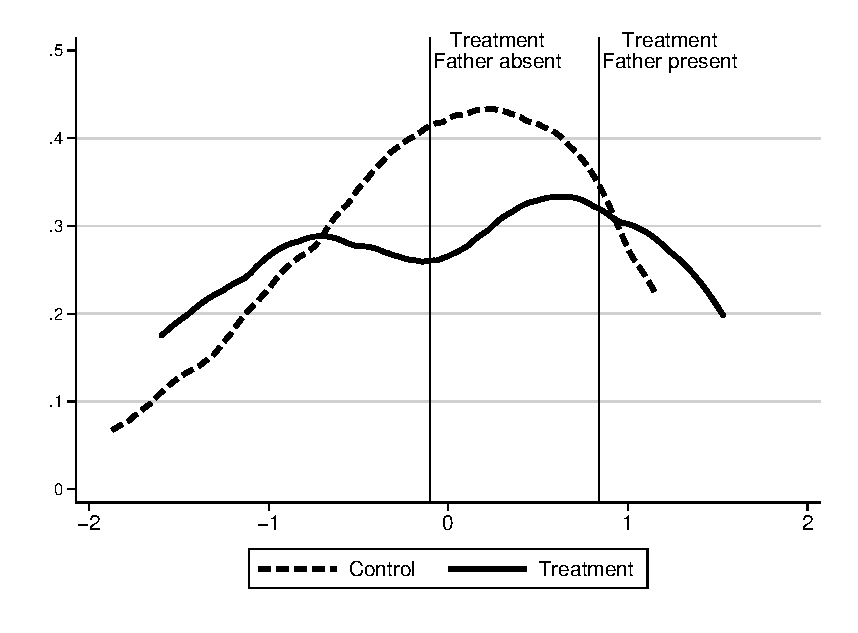
\includegraphics[width=\textwidth]{../output/HOME-males-factorhome}
	\end{subfigure}
	\begin{subfigure}[b]{0.49\textwidth}
		\centering
		\caption{Factor HOME Scores, Females}
		\label{fig:home-female-factor}
			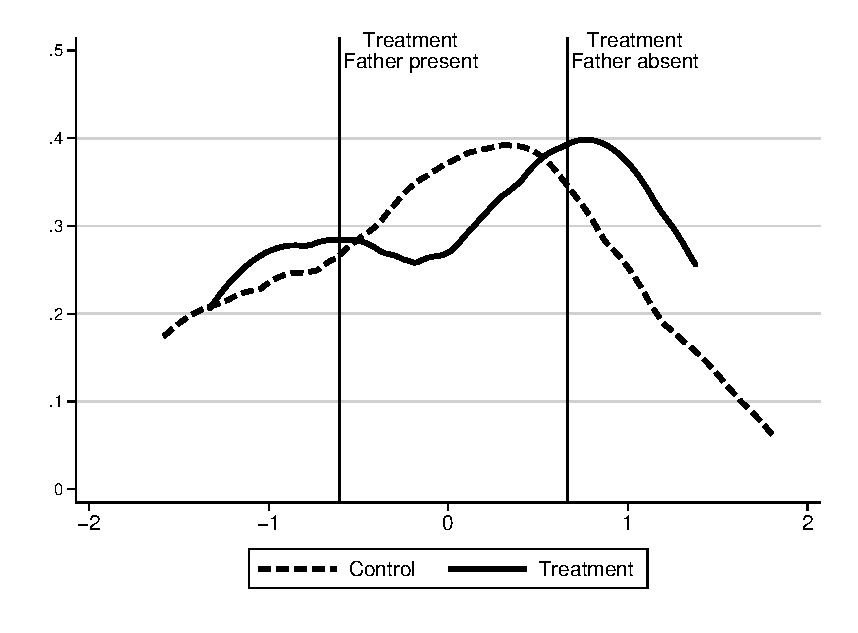
\includegraphics[width=\textwidth]{../output/HOME-females-factorhome}
	\end{subfigure}
\end{center}
\raggedright
Note: These plots show the distribution the factor of HOME scores. The factors are computed by gender using full HOME scores at 0.5, 1.5, 2.5, and 8 years. The vertical lines are the means of the treatment group by father's presence. 
\end{figure}

We explore this trend more closely in Figure~\ref{fig:total-home-quantiles}. To do so, we calculate the distribution pooling experimental groups but splitting by gender and father's presence. We then calculate, by gender and father's presence, the proportion of the treatment group that is in quantile 1 versus quantile 2. We do the same for the control group. 

The result of this exercise shows that the bimodal shape of the densities of the treatment group is explained differently by gender. For males, the HOME scores are higher for the control group when the fathers are absent and higher for the treatment group when father's are present. For females, the opposite is the case: The HOME scores are higher for the control group when fathers are present and higher for the treatment group when fathers are absent. 

One explanation of this is that treatment complements father's presence for males but substitutes it for females. Mothers then compensate for the father's absence for males (females) in the control (treatment) group. 

%One way mothers can compensate for the father's absence for males is to enroll them in alternate preschool arrangements. This is seen with more males in the control group being enrolled in these arrangements than control-group females (Figure~\ref{fig:alt-enrollment}). 

\begin{sidewaysfigure}
\begin{center}
\caption{Factor HOME Scores}
\label{fig:total-home-quantiles}
	\begin{subfigure}[b]{0.49\textwidth}
		\centering
		\caption{HOME, Father Absent, Males}
		\label{fig:home-male-mean}
			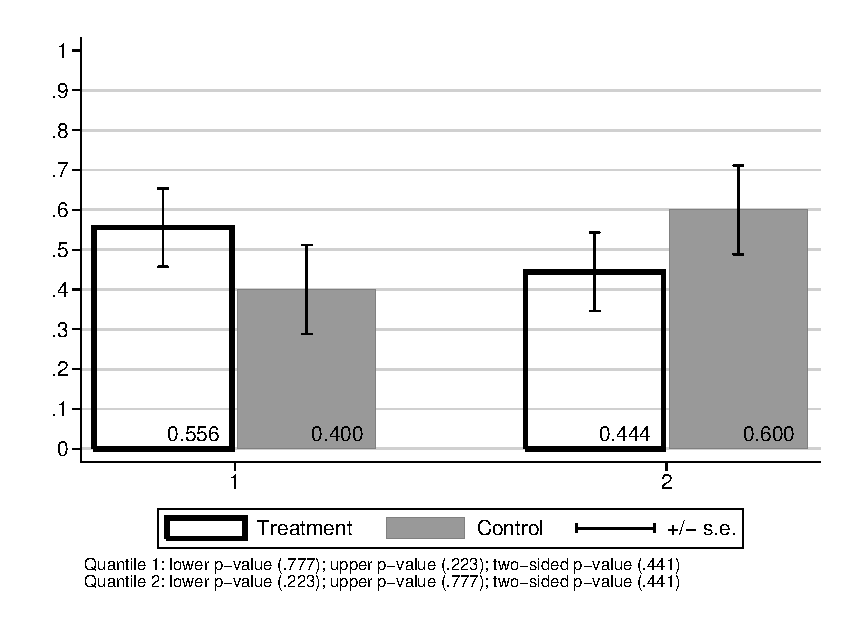
\includegraphics[width=\textwidth]{../output/HOME-male1-fhome0-2quant}
	\end{subfigure}
	\begin{subfigure}[b]{0.49\textwidth}
		\centering
		\caption{HOME, Father Absent, Females}
		\label{fig:home-female-mean}
			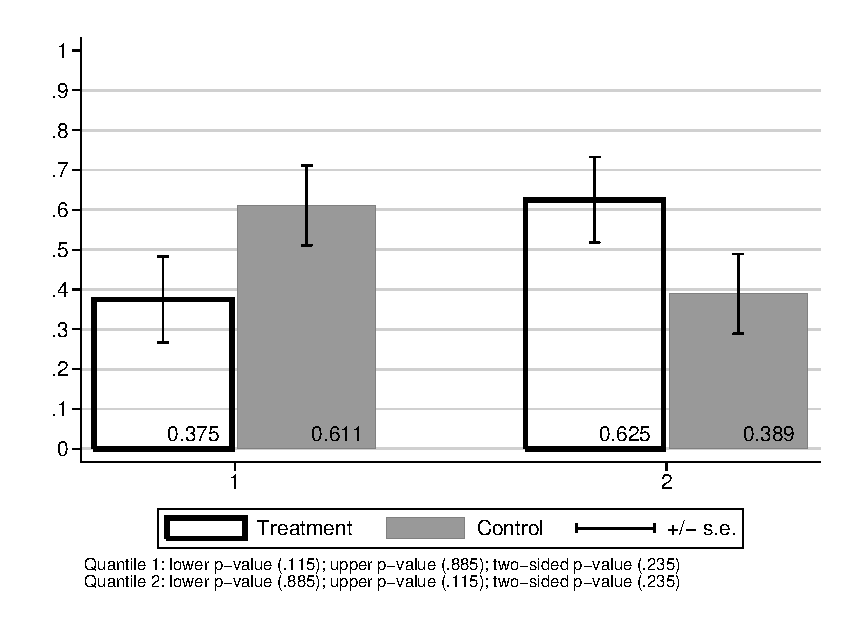
\includegraphics[width=\textwidth]{../output/HOME-male0-fhome0-2quant}
	\end{subfigure}
	
	\begin{subfigure}[b]{0.49\textwidth}
		\centering
		\caption{HOME, Father Present, Males}
		\label{fig:home-male-factor}
			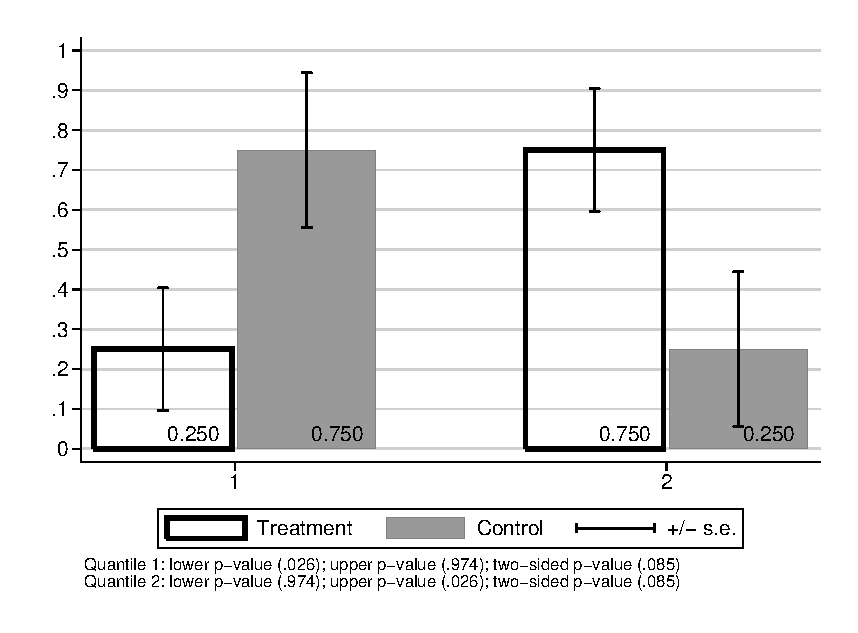
\includegraphics[width=\textwidth]{../output/HOME-male1-fhome1-2quant}
	\end{subfigure}
	\begin{subfigure}[b]{0.49\textwidth}
		\centering
		\caption{HOME, Father Present, Females}
		\label{fig:home-female-factor}
			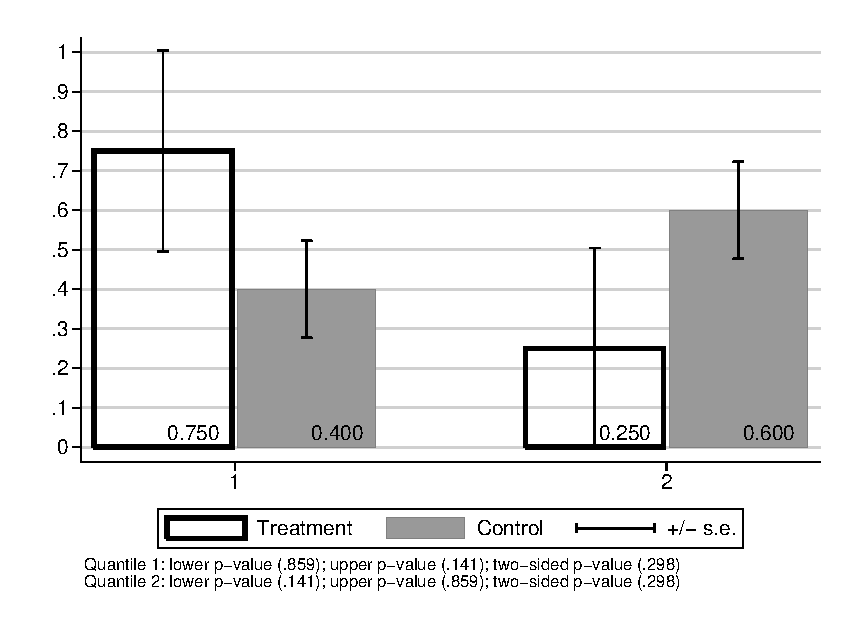
\includegraphics[width=\textwidth]{../output/HOME-male0-fhome1-2quant}
	\end{subfigure}
\end{center}
\raggedright \footnotesize
Note: The horizontal axis divides a factor of the HOME scores into the first and second quantile of the distribution pooling across experimental groups, but splitting  by gender and father's presence. The factors are computed by gender using full HOME scores at 0.5, 1.5, 2.5, and 8 years. The lower $p$-value tests that the treatment proportion is less than the control proportion within a quantile. The upper $p$-value tests that the treatment proportion is greater than the control proportion within a quantile. The numbers reported in the bars are the proportions. All standard errors and $p$-values are calculated using 1,000 bootstraps.
\end{sidewaysfigure}

%\begin{figure}
%\begin{center}
%\caption{Alternate Preschool Enrollment}
%\label{fig:alt-enrollment}
%	\begin{subfigure}[b]{0.49\textwidth}
%		\centering
%		\caption{Males by Father's Presence}
%			\includegraphics[width=\textwidth]{../output/family-dcmopre-father-male}
%	\end{subfigure}
%	\begin{subfigure}[b]{0.49\textwidth}
%		\centering
%		\caption{Females by Father's Presence}
%			\includegraphics[width=\textwidth]{../output/family-dcmopre-father-female}
%	\end{subfigure}
%	
%		\begin{subfigure}[b]{0.49\textwidth}
%		\centering
%		\caption{Pooled}
%			\includegraphics[width=\textwidth]{../output/family-dcmopre}
%	\end{subfigure}
%	\end{center}
%\raggedright
%Note: These histograms display the distributions of the months of enrollment in alternative preschool by gender. Months of enrollment are cumulative between birth and 5 years. 
%\end{figure}

\subsection{Adult Outcomes}

\begin{figure}[H]
\begin{center}
\caption{Crime}
\label{fig:}	
	\begin{subfigure}[b]{0.49\textwidth}
		\centering
		\caption{Felonies}
			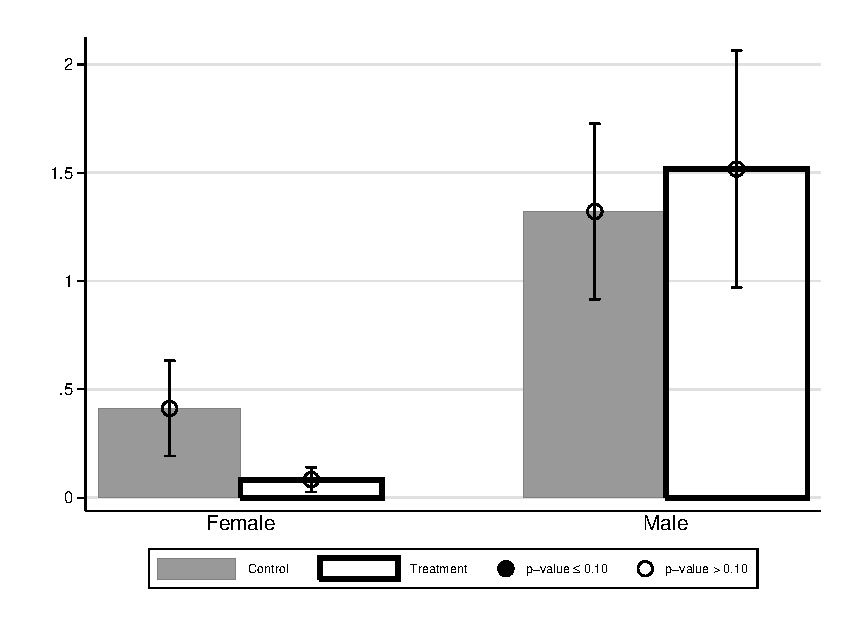
\includegraphics[width=\textwidth]{../output/Outcomes_Correlation/abccare/crime/bar-gender-trt-ad34_fel}
		\end{subfigure}
	\begin{subfigure}[b]{0.49\textwidth}
		\centering
		\caption{Misdemeanors}
			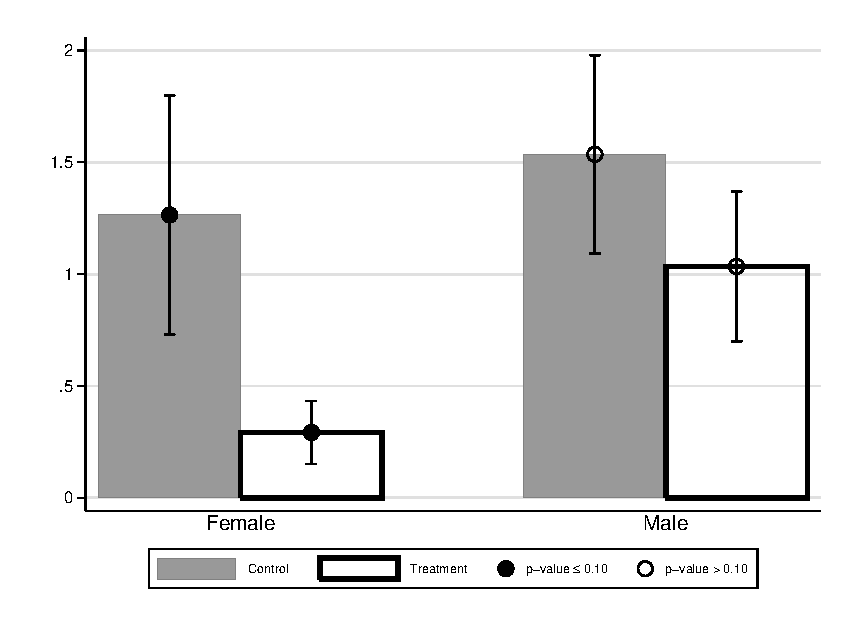
\includegraphics[width=\textwidth]{../output/Outcomes_Correlation/abccare/crime/bar-gender-trt-ad34_mis}
	\end{subfigure}
	\end{center}
\raggedright \footnotesize
Note:
\end{figure}

\begin{figure}[H]
\begin{center}
\caption{Age of First Crime}
\label{fig:age-first-crime}
	\includegraphics[width=\textwidth]{../output/Outcomes_Correlation/abccare/crime/bar-gender-trt-juv_crime_age}
\end{center}
\raggedright \footnotesize
Note:
\end{figure}		

\section{Mediation Analysis}
\label{sec:results}
To find a set of early, school-age, and adult mediators, we start by focusing on two life-cycle outcomes: labor income and savings in crime costs, both of which are in net present value of 2014 dollars discounted to birth of the subjects assuming a 3\% discount rate.\footnote{These outcomes are estimated following the methods described in \citet{Garcia_etal_2016_Comp_CBA_Unpublished}. These outcomes allow us to analyze the mediation beyond the ages observed at data collection. The inference for the following analysis accounts for the construction of the net present value of income, which uses an auxiliary sample to predict unobserved earnings. We bootstrap over the auxiliary sample in addition to bootstrapping over the ABC/CARE sample. The auxiliary data for crime is the complete population of individuals who committed crimes in North Carolina.}

We first estimate the effect of the early mediators, $\bm{\theta^E}$, on the school-age mediators, $\bm{\theta^S}$. In this case, $\bm{\theta^E}$ and $\bm{\theta^S}$ are vectors containing cognitive, non-cognitive, and parenting skills. For each $\theta^E_s$ in $\bm{\theta^S}$, we calculate

\begin{equation}
	\theta^S_s = \alpha_0 +\bm{ \alpha} \bm{\theta^E} + \varepsilon.
\end{equation}

Then, we estimate the effect of the school-age mediators on the adult mediators, $\bm{\theta^A}$. For each $\theta^A_a$ in $\bm{\theta^A}$, we calculate:

\begin{equation}
	\theta^A_a = \mu_0 + \bm{\mu} \bm{\theta^S} + \epsilon.
\end{equation}

Finally, we estimate the effect of the later mediators on the outcome of interest, $Y$:

\begin{equation}
	Y = \gamma_0 +\bm{\gamma} \bm{\theta^A} + \nu. 
\end{equation}

All of the parameters in these equations are estimated in the full sample of ABC/CARE. That is, we impose that the technology is the same across genders. We then split the sample by gender to calculate the treatment effect and decompose it based on the inputs of the above equations. To get the proportions reported below, we multiply this treatment effect by the estimates of the corresponding parameters from the above equations, and divide by the total treatment effect. This is a standard Laspeyres decomposition.

A pattern that emerges when considering the early and school-age skills as mediators is that cognitive skills tend to mediate for females more so than for males, and that the reverse is true for non-cognitive and parenting skills.

\begin{figure}[H]
\begin{center}
\caption{Early Skills on School-age Non-cognitive Skills}
\label{fig:earlyskills-ncog}
	\includegraphics[width=\textwidth]{../output/mediation/ncogfactor-nch-1-1-1}
\end{center}
\raggedright
Note: 
\end{figure}


\begin{figure}[H]
\begin{center}
\caption{Early Skills on School-age Retention}
\label{fig:earlyskills-retention}
	\includegraphics[width=\textwidth]{../output/mediation/never_ret-nch-1-1-1}
\end{center}
\raggedright
Note: 
\end{figure}


\begin{figure}[H]
\begin{center}
\caption{School-age Skills on Years of Education}
\label{fig:schoolskills-years}
	\includegraphics[width=\textwidth]{../output/mediation/years_30y-ncr-1-1-1}
\end{center}
\raggedright
Note: 
\end{figure}


\begin{figure}[H]
\begin{center}
\caption{School-age Skills on College Graduation}
\label{fig:schoolskills-univ}
	\includegraphics[width=\textwidth]{../output/mediation/si30y_univ_comp-ncr-1-1-1}
\end{center}
\raggedright
Note: 
\end{figure}

\begin{figure}[H]
\begin{center}
\caption{High School Graduation on Lifetime Income}
\label{fig:hs-npvincome}
	\includegraphics[width=\textwidth]{../output/mediation/income-s-1-1-1}
\end{center}
\raggedright
Note: 
\end{figure}

\begin{figure}[H]
\begin{center}
\caption{High School Graduation on Lifetime Crime Savings}
\label{fig:hs-npvcrime}
	\includegraphics[width=\textwidth]{../output/mediation/crime-s-1-1-1}
\end{center}
\raggedright
Note: 
\end{figure}


%\section{Summary}
%\label{sec:conclusion}
%When considering the early and school-age skills mediating educational attainment, we find that non-cognitive skills are significant mediators for both males and females. Given the importance of educational attainment in mediating other adult outcomes, the fact that non-cognitive skills are mediators for it highlights the dynamic importance of the non-cognitive skills. 
The proportion of the treatment effect explained by the skills do not differ by gender. Instead, the treatment effects for years of education are much larger for females than for males. 

Gender differences also appear when considering educational attainment as a mediator for labor income. At age 30, years of education is a negative mediator of labor income for females. This indicates that more educated women are staying at home, i.e., although treatment may increase years of education, that in turn does not necessarily lead to a full-time career by age 30. However, when considering the lifetime income, we find that the educational attainment has the opposite effect. In this case, educational attainment for females positively mediates labor income. It is striking to compare these results to those of the males, in which educational attainment is not a significant mediator income for neither the age-30 nor the lifetime income. Although females may exit the labor force during their child-bearing years, they re-enter and recover income through their increased educational attainment. 

Finally, we consider crime savings to explore another way in which educational attainment can mediate the adult treatment effects. For females, years of schooling mediate a large proportion of the crime savings, as is consistent with the findings in \citet{Heckman_Pinto_etal_2013_PerryFactor} for subjects in the Perry Preschool Project (Perry). There are two justifications for this similarity. One reason is that the females in ABC/CARE commit similar crimes to the Perry subjects. Relative to the ABC/CARE males, ABC/CARE female subjects commit more non-violent crimes than violent ones. Another reason is that the males begin committing crimes earlier, in turn precluding further educational attainment.

These results reveal the importance of non-cognitive skills, not only on later mediators like educational attainment, but also on adult outcomes of interest. Although there are not gender differences on the importance of these skills on educational attainment, there are gender differences on educational attainment's mediation of labor income and crime savings.  
	

\clearpage
\singlespacing
\bibliography{heckman}
\bibliographystyle{chicago}

\end{document}
